\documentclass[12pt,a4paper]{article}
% Estilo compartido para informes. Compilar con LuaLaTeX desde tp1/.
\usepackage[spanish,es-nodecimaldot]{babel}
\usepackage{fontspec}
\setmainfont{Montserrat-Medium.ttf}[
  Path=../assets/fonts/,
  BoldFont=Montserrat-Bold.ttf,
  ItalicFont=Montserrat-MediumItalic.ttf]
\usepackage[a4paper,margin=2.5cm,headheight=16pt]{geometry}
\usepackage{xcolor,graphicx,booktabs,tabularx}
\usepackage{float}
\usepackage{titlesec,fancyhdr,enumitem,caption}
\usepackage{ragged2e}
\usepackage{hyperref}
\definecolor{verde}{HTML}{1D4036}
\definecolor{bronce}{HTML}{D38129}
\definecolor{rosa}{HTML}{D88E77}
\definecolor{calido}{HTML}{EFE4D8}
\definecolor{grafito}{HTML}{1D1D1D}
\hypersetup{colorlinks=true,linkcolor=verde,urlcolor=verde,
  pdftitle={TP1 - Instalación de máquinas virtuales},pdfsubject={Cyberseguridad}}
\AtBeginDocument{\color{grafito}\RaggedRight\fontsize{12}{14.4}\selectfont}
\setlength{\parindent}{0pt}
\setlength{\parskip}{7pt}
\setlist[itemize]{leftmargin=*,itemsep=7pt,topsep=4pt}
\setlist[enumerate]{leftmargin=*,itemsep=6pt}
\titleformat{\section}{\color{verde}\bfseries\fontsize{18}{21.6}\selectfont}{\thesection}{0.65em}{}
\titleformat{\subsection}{\color{verde}\bfseries\large}{\thesubsection}{0.65em}{}
\titleformat{\subsubsection}{\color{verde}\bfseries}{\thesubsubsection}{0.65em}{}
\titlespacing*{\section}{0pt}{16pt}{8pt}
\titlespacing*{\subsection}{0pt}{12pt}{5pt}
\titlespacing*{\subsubsection}{0pt}{10pt}{4pt}
\setcounter{tocdepth}{2}
\pagestyle{fancy}
\fancyhf{}
\fancyhead[L]{\small\color{verde}FCEFyN | UNC}
\fancyhead[R]{\small\color{verde}\materia\ · TP \numeroTP}
\fancyfoot[L]{\scriptsize Informe de laboratorio}
\fancyfoot[R]{\small\thepage}
\renewcommand{\headrulewidth}{0.4pt}
\captionsetup{font=small,labelfont=bf,justification=raggedright,singlelinecheck=false,hypcap=false}
\newcommand{\pendiente}[1]{\par{\small\color{verde}\textbf{Por completar.} #1\par}}
% Si falta una captura se muestra un espacio reservado; no impide compilar.
\newcommand{\captura}[2]{%
  \par\smallskip\begingroup\centering
  \IfFileExists{figuras/#1}{%
    \includegraphics[width=\linewidth,height=5cm,keepaspectratio]{figuras/#1}%
  }{%
    \setlength{\fboxsep}{10pt}%
    \fcolorbox{bronce}{calido}{\parbox[c][1.25cm][c]{\dimexpr\linewidth-2\fboxsep-2\fboxrule\relax}{%
      \centering\small Captura pendiente\par\texttt{\detokenize{#1}}}}%
  }%
  \captionof{figure}{#2}\par\endgroup\smallskip
}

\usepackage{xurl}

\newcommand{\materia}{Cyberseguridad}
\newcommand{\numeroTP}{9}
\newcommand{\tituloTP}{Firma digital de correos}
\newcommand{\estudiante}{Brigido Tomas Andres}
\newcommand{\legajo}{38481096}
\newcommand{\carrera}{ICOMP}
\newcommand{\docente}{Javier A. Jorge}


% Metadatos específicos del TP9 y capturas en img/.
\hypersetup{pdftitle={TP9 - Firma digital de correos}}
\renewcommand{\captura}[2]{%
  \begin{figure}[H]
    \centering
    \IfFileExists{img/#1}{%
      \includegraphics[width=0.85\linewidth,height=5cm,keepaspectratio]{img/#1}%
    }{%
      \setlength{\fboxsep}{10pt}%
      \fcolorbox{bronce}{calido}{\parbox[c][1.1cm][c]{0.85\linewidth}{%
        \centering\small Captura pendiente\par\texttt{\detokenize{#1}}}}%
    }%
    \caption{#2}
  \end{figure}
}

\begin{document}
\hypersetup{pageanchor=false}
\begin{titlepage}
  
\includegraphics[width=8cm]{../assets/logo-fcefyn-2026.png}
  \vspace{1cm}

  {\color{verde}\small UNIVERSIDAD NACIONAL DE CÓRDOBA\par}
  \vspace{2.1cm}
  {\color{bronce}\bfseries\large TRABAJO PRÁCTICO \numeroTP\par}
  \vspace{0.45cm}
  {\color{verde}\bfseries\fontsize{32}{38.4}\selectfont Firma digital\\de correos\par}
  \vspace{0.3cm}
{\small OpenPGP y certificados para correo electrónico\par}
\vspace{0.35cm}
  {\large \materia\par}
  \vspace{0.8cm}
  {\color{bronce}\rule{2.7cm}{2pt}\par}
  \vfill
  \renewcommand{\arraystretch}{1.45}
  \begin{tabular}{@{}p{3.2cm}p{10cm}@{}}
    Estudiante & \estudiante \\
    Legajo & \legajo \\
    Carrera & \carrera \\
    Docente & \docente \\
  \end{tabular}
  \vfill
  {\small Córdoba, Argentina\par}
\end{titlepage}
\hypersetup{pageanchor=true}

\tableofcontents
\vspace{1cm}
\newpage

\section{Introducción y objetivos}
Esta actividad propone utilizar Thunderbird con el correo universitario para firmar y cifrar mensajes. Se documentará la generación e intercambio de claves OpenPGP y el uso de un certificado de terceros, siguiendo la consigna.

\section{Generación del par de claves OpenPGP}

\begin{figure}[H]
    \centering
    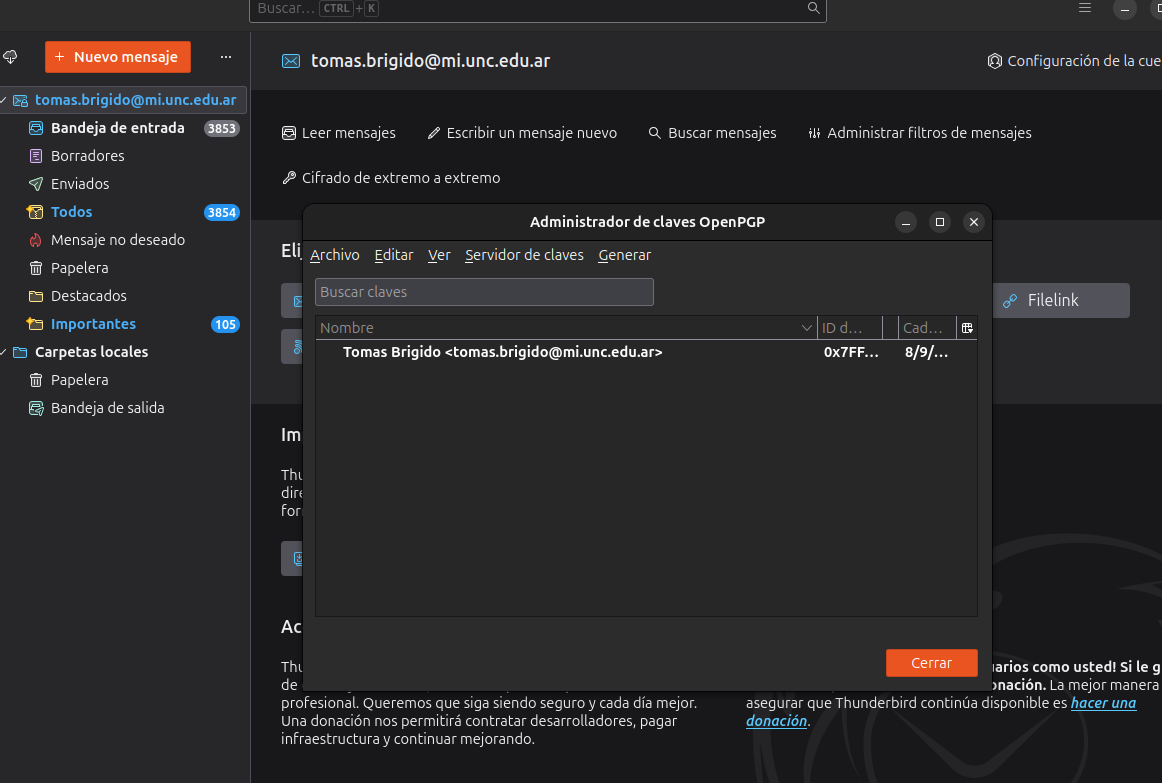
\includegraphics[width=0.9\textwidth]{img/clavegenerada.png}
    \caption{Par de claves OpenPGP generado.}
    \label{fig:captura-dns}
\end{figure}

\section{Intercambio y selección de la clave}

\begin{figure}[H]
    \centering
    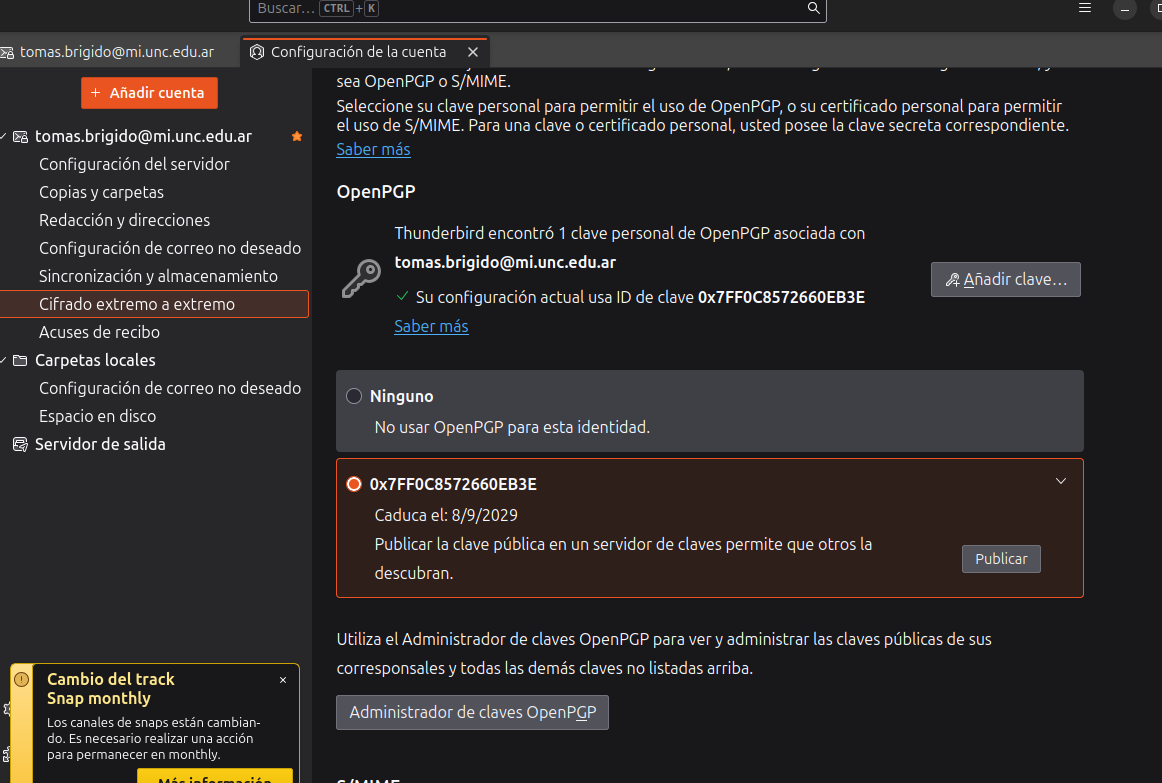
\includegraphics[width=0.9\textwidth]{img/end2end.png}
    \caption{Configuración de cifrado de extremo a extremo.}
    \label{fig:captura-dns}
\end{figure}

\section{Envío de mensajes firmados y cifrados}
\textbf{Mensaje firmado y cifrado .}

\begin{figure}[H]
    \centering
    \begin{minipage}{0.48\textwidth}
        \centering
        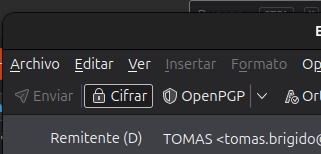
\includegraphics[width=\linewidth]{img/cifradoyopenpgp.png}
        \caption{Mensaje firmado y cifrado con OpenPGP.}
        \label{fig:imagen1}
    \end{minipage}
    \hfill
    \begin{minipage}{0.48\textwidth}
        \centering
        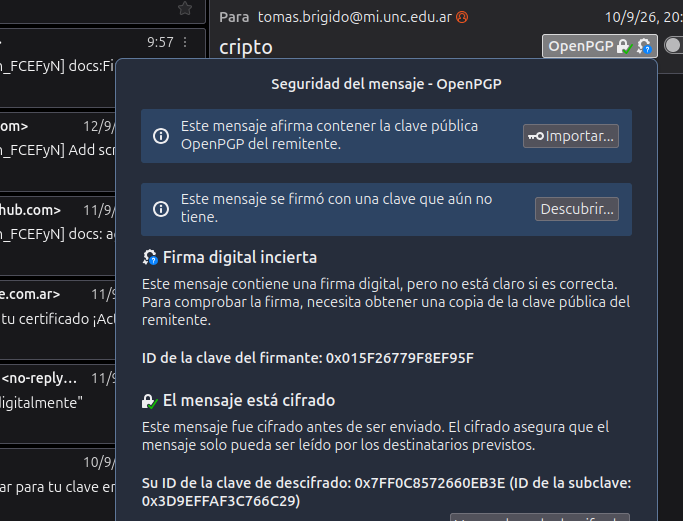
\includegraphics[width=\linewidth]{img/msgcifrado.png}
        \caption{Mensaje recibido y descifrado.}
        \label{fig:imagen2}
    \end{minipage}
\end{figure}

\newpage
\section{Referencias}
\begin{itemize}
  \item \textit{Criptografía y seguridad 2022: Firma digital de correos electrónicos}. Consigna local: \textit{firmadigital de correos.pdf}.
  \item \href{https://www.howtogeek.com/706402/how-to-use-openpgp-encryption-for-emails-in-thunderbird/}{How to Use OpenPGP Encryption for Emails in Thunderbird}. Lectura indicada en la consigna.
  \item \href{https://keys.openpgp.org/}{keys.openpgp.org}. Servidor de claves indicado en la consigna.
  \item \href{https://www.dannyguo.com/blog/how-to-get-a-free-s-mime-certificate/}{How to Get a Free S/MIME Certificate}. Lectura indicada en la consigna.
\end{itemize}
\end{document}
